\newcommand{\defaultparindent}{\parindent}
\setlength{\parindent}{0pt}				% \noindent partout
% \parindent in one-column documents is :
% 15pt when the default text size is 10pt,
% 17pt for 11pt,
% and 1.5em for 12pt.
% In two-column documents it is 1em

\begin{center}
\begin{tabular}{p{5cm} p{11cm}}
\textbf{Commandes étudiées :} & \texttt{sh}, \texttt{bash}, \texttt{man}, \texttt{ls}, \texttt{mkdir}, \texttt{touch}, \texttt{chmod}, \texttt{mv}, \texttt{rm}, \texttt{rmdir}, \texttt{cat}, \texttt{file}, \texttt{whereis}, \texttt{which}\\

\textbf{Builtins étudiées :} & \texttt{pwd}, \texttt{cd}, \texttt{exit}, \texttt{logout}, \texttt{echo}, \texttt{umask}, \texttt{type}, \texttt{>}, \texttt{>{}>}, \texttt{<}, \texttt{<{}<}, \texttt{|}\\

\textbf{Notions étudiées :} & Shell, Manuels, Fichiers, Répertoires, Droits, Redirections\\
\end{tabular}
\end{center}

\bigskip

\subsection{Lancement et Manuels}

\bigskip

Le shell est un programme permettant d'interpréter et d'exécuter des actions à partir de commandes écrites par l'utilisateur.
Concrètement, dans le cas du shell d'un système d'exploitation, il s'agit d'un programme permettant de lancer des programmes selon ce que l'utilisateur demande.
Les shells actuels permettent de chaîner des programmes et potentiellement faire d'autres actions (comme rediriger les messages d'erreur vers des fichiers, conditionner le lancement de certains programmes, etc).

\bigskip

Sur UNIX, il existe historiquement deux familles de shells :
\begin{itemize}
\item les dérivés du \textit{bourne shell} (sh) : bash (Bourne again shell), ksh (Korn shell), zsh, ...
\item les \textit{C-shells} (en voie de disparition) : csh, tcsh
\end{itemize}

D'autres shells plus récents sont également apparus, mais nous ne les étudierons pas.
Il faut principalement retenir que le langage reconnu par les \textit{bourne shells} n'est absolument pas reconnu par les \textit{C-shells}.
Mais n'importe quel script écrit pour \textit{sh} sera reconnu et interprété correctement par \textit{bash}, \textit{ksh}, \textit{zsh}, ...

Il est important de comprendre la différence entre le \textbf{langage} que vous écrivez, et le \textbf{programme} qui le lit : une implémentation différente engendrera parfois des comportements différents pour une même instruction.
Dit autrement, deux programmes différents peuvent reconnaître le même langage, mais ne pas effectuer strictement les mêmes opérations (par exemple, il existe deux façons d'implémenter la multiplication, mais leurs résultats restent les mêmes : pour $ n \times m $, on peut faire $ n $ additions de $ m $ [ $ m + m + ... + m $ ], ou $ m $ additions de $ n $ [ $ n + n + ... + n $ ]).

\bigskip

On pourra noter que les entreprises utilisent le \textit{Korn shell} étant donné que des implémentations payantes de celui-ci sont vendues et maintenues.
Il existe néanmoins quelques implémentations gratuites et libres : \textit{mksh}, \textit{pdksh} (Public Domain ksh), ...
On pourra noter que le \textit{ksh} étant certifié POSIX, il est possible de le compiler puis l'exécuter sur n'importe quel système conforme à POSIX (donc Windows peut potentiellement lire et exécuter des scripts écrits pour \textit{sh}).

\bigskip

Intéressons-nous maintenant aux commandes classiques sur les UNIX/Linux.
Le tableau~\ref{table:Cours-TableauCommandesClassiques} montre les commandes habituellement utilisées dans le shell, et qui correspondent à ce que vous feriez avec une interface graphique.

\begin{table}[h!]
\centering
\begin{tabular}{| l | L{10cm} |}
\hline
Commande & Description \\
\hline
\TTBF{ls} & Lister le contenu d'un répertoire \\ \hline
\TTBF{cp} & Copier un fichier \\ \hline
\TTBF{mv} & Déplacer un fichier \\ \hline
\TTBF{rm} & Supprimer un fichier \\ \hline
\TTBF{ln} & Créer un lien (dur ou symbolique) vers un fichier ou un répertoire \\ \hline
\TTBF{mkdir} & Créer un répertoire \\ \hline
\TTBF{rmdir} & Supprimer un répertoire \\ \hline
\TTBF{cd} & Changer de répertoire courant \\ \hline
\TTBF{pwd} & Afficher le chemin complet du répertoire courant \\ \hline
\end{tabular}
\caption{Commandes classiques sur UNIX/Linux}
\label{table:Cours-TableauCommandesClassiques}
\end{table}

Connectez-vous sur une machine, et lancer un terminal. Lorsque celui-ci est lancé, quelques lignes devraient s'afficher dedans, il s'agit du \textbf{prompt}.\\

Il y a plusieurs prompts par défaut, voici une liste non exhaustive :\\

\TTBF{\$} \\
\TTBF{\%} \\
\TTBF{>} \\
\TTBF{bash\$>} \\

L'utilité du prompt est de savoir si le shell vous offre la posibilité de taper des commandes, ou s'il est en train d'effectuer un traitement.
Vous pouvez le personnaliser pour qu'il affiche des informations utiles (l'heure, la date, le dossier où vous vous trouvez, ...).\\

\bigskip

Pour démarrer, apprenez à vous servir de la commande \texttt{man} (pour manuel).\\

\TTBF{man man}\\

Une documentation apparaitra, vous pouvez vous déplacer dedans avec les touches fléchées, et quitter en appuyant sur la touche 'q'.
Pour bien utiliser les manuels, indiquez en argument la commande que vous souhaitez étudier.
Par exemple, pour se documenter sur \texttt{ls}, tapez :\\

\TTBF{man ls}\\

Pour se documenter sur la commande shell/builtin \texttt{printf}, il faut demander explicitement la section 1 du manuel.\\

\TTBF{man 1 printf}\\

Pour se documenter sur la fonction C \texttt{printf}, il faut demander explicitement la section 3 du manuel.\\

\TTBF{man 3 printf}\\

Dans le même cas, pour se documenter sur l'appel système (syscall) \texttt{read}, utilisez la section 2 du manuel.\\

\TTBF{man 2 read}\\

Par défaut, \texttt{man} essaye d'utiliser la section la plus petite pour l'argument qu'on lui donne (\texttt{read} dispose des sections 1 et 2, mais \texttt{lseek} ne dispose pas de section 1) :\\

\TTBF{man read}\\
\TTBF{man lseek}\\

Une autre commande est également utilisé dans le monde du GNU : \texttt{info}.
Celle-ci donne des informations sur la version GNU des outils, et est beaucoup plus complète dans certains cas.\\

\TTBF{info ls}\\

Pour quitter le shell et fermer sa session, utilisez les commandes \texttt{exit} ou \texttt{logout}.\\

\bigskip


\newpage
%%%%%%%%%%%%%%%%%%%%%%%%%%%%%%%%%%%%%%%%%%%%%%%%%%%%%%%%%%%%%%%%%%%%%%%%%%%%%%%%
\subsection{Déplacement dans le Shell}

\bigskip

Pour connaitre votre position dans l'arborescence, utilisez la commande \texttt{pwd}.\\

\TTBF{pwd}\\

Le chemin absolu va s'afficher. Il s'agit du chemin depuis la racine de l'arborescence.\\

\bigskip

Pour connaitre les fichiers et dossiers présents là où vous vous trouvez, utilisez la commande \texttt{ls}.\\

\TTBF{ls}\\

%Pour avoir plus de détails, et lister un fichier par ligne, utilisez le paramètre \TTBF{-l}.
Pour connaitre les \textbf{droits} et d'autres propriétés de chaque élément, tout en listant un fichier par ligne, utilisez l'option \texttt{-l} (lettre L).\\

\TTBF{ls -l}\\

\bigskip

Le paramètre \TTBF{-a} affiche les fichiers et dossiers considérés comme cachés (c'est-à-dire commençant par un point \TTBF{.}).

\TTBF{le -l -a}

\bigskip

On peut combiner les paramètres \TTBF{-a} et \TTBF{-l} ainsi : \TTBF{ls -la} pour pouvoir afficher l'ensemble des fichiers et dossiers contenus dans un répertoire, le tout un fichier par ligne, et avec le maximum d'informations possibles.\\

\TTBF{ls -la}\\

\bigskip

Vous allez créer un dossier/répertoire nommé "MonDossier" en utilisant la commande \texttt{mkdir}.\\

\TTBF{mkdir MonDossier}\\

Pour vous déplacer dans ce dossier, utilisez la commande/builtin \texttt{cd}.\\

\TTBF{cd MonDossier}\\

\bigskip

Maintenant, observez le nouveau chemin absolu.\\

\TTBF{pwd}\\

Deux dossiers sont toujours présents dans \textit{tous} les dossiers, affichez-les en utilisant l'option \texttt{-a} de \texttt{ls}.\\

\TTBF{ls -a}\\

Le dossier "." correspond au dossier courant, le dossier ".." correspond au dossier parent.
Essayez donc ces deux commandes en testant le chemin absolu :\\

\TTBF{cd .}\\
\TTBF{pwd}\\
\TTBF{cd ..}\\
\TTBF{pwd}\\

Allez dans le dossier \textit{/bin} avec \texttt{cd}, et regardez le chemin absolu.\\

\TTBF{cd /bin}\\
\TTBF{pwd}\\

Essayez maintenant d'utiliser la commande/builtin \texttt{cd} sans argument, et regardez où vous vous trouvez.\\

\TTBF{cd}\\
\TTBF{pwd}\\

Il s'agit de votre \textbf{home directory}, celui qui vous est alloué pour vos fichiers et dossiers.
Lorsque \texttt{cd} est utilisé sans argument, vous revenez automatiquement à votre dossier utilisateur/home directory.\\
Essayez maintenant d'utiliser la commande/builtin \texttt{cd} avec l'argument \texttt{-}.\\

\TTBF{cd -}\\
\TTBF{pwd}\\

Vous vous retrouvez dans le dossier \textit{précédent}.
Il ne s'agit pas du dossier parent, mais du dossier où vous étiez précédemment (si vous avez utilisez des chemins absolus, vous serez déplacés vers l'ancien répertoire).\\

Retournez dans le dossier "MonDossier" que vous avez créé dans votre home directory.\\

\TTBF{cd \textasciitilde{}/MonDossier}\\

Le \texttt{\textasciitilde} (tilde) correspond à votre dossier utilisateur/home directory.\\

Créez ici deux dossiers : "Dossier1" et "Dossier2".\\

\TTBF{mkdir Dossier1 Dossier2}\\
\TTBF{cd Dossier1}\\
\TTBF{pwd}\\

\bigskip

Il est possible d'enchaîner les chemins :\\

\TTBF{cd ../Dossier2}\\
\TTBF{pwd}\\
\TTBF{cd /usr/bin/../../etc}\\
\TTBF{pwd}\\

\bigskip


\newpage
%%%%%%%%%%%%%%%%%%%%%%%%%%%%%%%%%%%%%%%%%%%%%%%%%%%%%%%%%%%%%%%%%%%%%%%%%%%%%%%%
\subsection{Fichiers, Répertoires, et Droits}

\bigskip

\TTBF{cd \textasciitilde{}/MonDossier}\\

Il est possible de créer des fichiers vides, s'ils étaient inexistants, grâce à la commande \texttt{touch}.\\

\TTBF{ls -la}\\
\TTBF{touch MonFichier}\\
\TTBF{ls -la}\\

L'option \texttt{-l} de \texttt{ls} permet d'afficher les droits et d'autres informations.
La commande \texttt{chmod} permet de modifier ces droits.\\

\TTBF{chmod 755 MonFichier}\\
\TTBF{ls -la}\\
\TTBF{chmod 640 MonFichier}\\
\TTBF{ls -la}\\

Pour rappel, les droits sous forme de nombres correspondent à : \textit{Propriétaire-Groupe-Autres} sous forme de combinaison (1 droit d'\textit{exécution}, 2 droit d'\textit{écriture}, 4 droit de \textit{lecture}).
Le droit d'exécution permet aux dossiers d'être accessibles, et aux fichiers d'être lancés.\\

\bigskip

La commande \texttt{echo} permet d'afficher du texte.\\

\TTBF{echo "Coucou !"}\\

Afin de remplir le fichier, nous allons utiliser un opérateur de redirection \texttt{>} pour transférer les données écrites par \texttt{echo} vers le fichier "MonFichier" (nous verrons plus tard les détails).\\

\TTBF{echo "Coucou !" > MonFichier}\\

La commande \texttt{cat} permet d'afficher le contenu d'un fichier passé en paramètre (mais pas seulement...).\\

\TTBF{cat MonFichier}\\

Testons les droits de nouveau.\\

\TTBF{chmod 000 MonFichier}\\
\TTBF{cat MonFichier}\\

\TTBF{chmod 400 MonFichier}\\
\TTBF{echo "A" > MonFichier}\\
\TTBF{cat MonFichier}\\

\TTBF{chmod 200 MonFichier}\\
\TTBF{echo "B" > MonFichier}\\
\TTBF{cat MonFichier}\\

\TTBF{chmod 640 MonFichier}\\
\TTBF{echo "C" > MonFichier}\\
\TTBF{cat MonFichier}\\

\bigskip

L'option \texttt{-e} de \texttt{echo} permet d'interpréter certains caractères tels que \texttt{\textbackslash n} ou encore \texttt{\textbackslash t}.\\

\TTBF{echo -e "Ceci\textbackslash nest\textbackslash nun\textbackslash ntest." > MonFichier}\\
\TTBF{cat MonFichier}\\

Vérifiez le droit d'exécution avec les tests suivants (attention aux guillemets " et ').
Pour exécuter un fichier, il suffit de le préfixer de \texttt{./} comme dans l'exemple \texttt{./script.sh}.\\

\TTBF{echo -e \textquotesingle \#! /bin/sh\textbackslash n\textbackslash necho "Ca marche"\textbackslash n\textquotesingle {} > MonFichier}\\

\TTBF{chmod 750 MonFichier}\\
\TTBF{cat MonFichier}\\
\TTBF{./MonFichier}\\

\TTBF{chmod 640 MonFichier}\\
\TTBF{cat MonFichier}\\
\TTBF{./MonFichier}\\

\TTBF{chmod 100 MonFichier}\\
\TTBF{cat MonFichier}\\
\TTBF{./MonFichier}\\

\TTBF{chmod 750 MonFichier}\\

La commande \texttt{umask} permet de modifier les droits par défaut lors de la création d'un fichier ou répertoire.
\texttt{umask} prend en paramètre un nombre similaire à celui de \texttt{chmod}, mais celui-ci sera l'inverse des droits donnés.
Précisément, il s'agit d'un masque filtrant les droits demandés : donner \texttt{777} à \texttt{umask} signifie que tous les droits seront filtrés (et interdits), donc que l'équivalent d'un \texttt{chmod 000} est appliqué.
À l'inverse, un \texttt{umask 000} signifie que l'on ne filtre aucun droit, donc que les nouveaux fichiers peuvent être créés avec n'importe quels droits.
%Par exemple, donner \texttt{777} à \texttt{umask} signifie qu'un \texttt{chmod 000} est appliqué à tous les fichiers créés, inversement \texttt{umask 000} signifie appliquer un \texttt{chmod 777} à tous les nouveaux fichiers.
De façon plus pragmatique, un \texttt{umask 022} semble correct, car il acceptera au maximum un \texttt{chmod 755} sur les fichiers créés.\\

\TTBF{umask}\\
\TTBF{umask 777}\\
\TTBF{touch TestMask1}\\
\TTBF{ls -la}\\
\TTBF{umask 022}\\
\TTBF{touch TestMask2}\\
\TTBF{ls -la}\\
\TTBF{umask 077}\\
\TTBF{touch TestMask3}\\
\TTBF{ls -la}\\
\TTBF{umask 022}\\

\bigskip

Il est possible de déplacer un fichier ou un dossier avec la commande \texttt{mv}.\\

\TTBF{mv MonFichier ..}\\
\TTBF{mv ../MonFichier .}\\

Un autre effet de la commande \texttt{mv} est de renommer les fichiers.\\

\TTBF{mv MonFichier script.sh}\\

Pour supprimer un fichier, il faut utiliser \texttt{rm}.
En ajoutant \texttt{-i}, on demandera toujours une confirmation avant la suppression.
Inversement, pour forcer la suppression OU ignorer les erreurs, on peut utiliser l'option \texttt{-f}.\\

\TTBF{touch test1}\\
\TTBF{rm -i test1}\\
\TTBF{rm test1}\\
\TTBF{rm -f test1}\\
\TTBF{touch test1}\\
\TTBF{rm -f test1}\\

Pour supprimer un dossier, il faut utiliser \texttt{rmdir} si et seulement si le dossier est vide, ou alors utiliser \texttt{rm -f}.\\

\TTBF{mkdir dir1}\\
\TTBF{rm dir1}\\
\TTBF{rmdir dir1}\\
\TTBF{mkdir dir1}\\
\TTBF{touch dir1/file}\\
\TTBF{rmdir dir1}\\
\TTBF{rm -rf dir1}\\

\bigskip
%\newpage

Entraînez-vous à créer cette arborescence avec ces droits :\\

\begin{center}
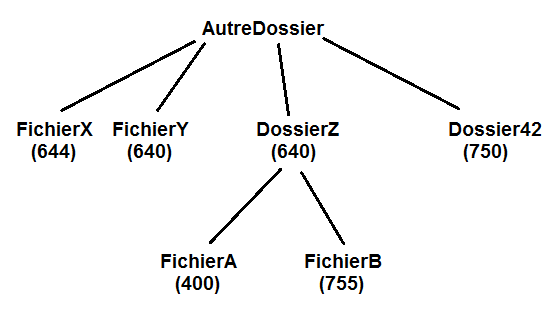
\includegraphics[scale=1]{Cours/TP1-arborescence.png}
\end{center}

Un équivalent de cette arborescence :\\

\TTBF{AutreDossier/}\\
\TTBF{AutreDossier/FichierX}\\
\TTBF{AutreDossier/FichierY}\\
\TTBF{AutreDossier/DossierZ/}\\
\TTBF{AutreDossier/DossierZ/FichierA}\\
\TTBF{AutreDossier/DossierZ/FichierB}\\
\TTBF{AutreDossier/Dossier42/}\\

\bigskip


\newpage
%%%%%%%%%%%%%%%%%%%%%%%%%%%%%%%%%%%%%%%%%%%%%%%%%%%%%%%%%%%%%%%%%%%%%%%%%%%%%%%%
\subsection{Types de Fichiers}

\bigskip

Il est possible d'identifier le type de fichier en utilisant la commande \texttt{file}.\\

\TTBF{file .}\\
\TTBF{file ../MonDossier}\\
\TTBF{echo "Coucou !" > MonTexte}\\
\TTBF{file MonTexte}\\
\TTBF{file MonFichier}\\

De la même manière, certaines commandes sont en réalités des sous-programmes/fonctions du shell et ne sont associées à aucun programme/binaire.
Par exemple \texttt{ls} est un programme indépendant, mais \texttt{cd} est une builtin du shell.
Pour identifier ces différences, plusieurs solutions existent : le manuel (voir si la manuel de la commande renvoie au manuel du shell/builtins), la commande \texttt{type} (builtin de bash), la commande \texttt{which}, la commande \texttt{whereis}.\\

\TTBF{man cd}\\
\TTBF{type cd}\\
\TTBF{which cd}\\
\TTBF{whereis cd}\\

\TTBF{man ls}\\
\TTBF{type ls}\\
\TTBF{which ls}\\
\TTBF{whereis ls}\\

Certaines commandes peuvent exister sous forme de binaire ET exister sous forme de builtin dans certains shells... dans ce cas, c'est la version shell qui primera (et il faudra appeler le programme avec son chemin long pour l'utiliser, par exemple : \texttt{/bin/ls}).\\

\bigskip


\newpage
%%%%%%%%%%%%%%%%%%%%%%%%%%%%%%%%%%%%%%%%%%%%%%%%%%%%%%%%%%%%%%%%%%%%%%%%%%%%%%%%
\subsection{Redirections (et File Descriptors)}

\bigskip

Dans le standard UNIX, pour transmettre des données en dehors d'un processus, on utilise des \textit{file descriptors}.
La philosophie UNIX se base sur un principe où \textit{tout est fichier}, et donc, la lecture ou l'écriture se fait via les primitives (ou syscalls) de traitement de fichiers (open, read, write, close, lseek, ...).
De plus, trois file descriptors sont constamment ouverts (sauf si leur manuel vous indique le contraire) : \textbf{STDIN} (0) Standard Input/l'entrée standard, \textbf{STDOUT} (1) Standard Output/la sortie standard, \textbf{STDERR} (2) Standard Error/la sortie d'erreur.
Chacun permet de lire un périphérique d'entrée, ou d'écrire vers un flux de sortie dédié aux erreurs ou aux informations normales.\\

\bigskip

Un premier exemple de redirection a été vu plus haut.\\

\TTBF{echo "Coucou" > File1}\\
\TTBF{cat File1}\\

Ici, nous avons demandé à rediriger la sortie standard vers le fichier "\textit{File1}".
On remarque facilement que rien n'a été écrit dans le terminal, mais que tout a été mis dans le fichier.
On peut étendre ce comportement à des commandes classiques :\\

\TTBF{ls -la > File1}\\
\TTBF{cat File1}\\

Inversement, lançez une commande qui échouera et écrira un message d'erreur (le fichier "\textit{inex}" n'existant pas) :\\

\TTBF{ls -l . inex > File1}\\
\TTBF{cat File1}\\

Un message d'erreur pour le fichier inexistant "\textit{inex}" s'affiche dans le terminal, et le fichier contient la sortie prévue pour \texttt{ls -l .}.
En effet, par défaut, seule la sortie standard est redirigée avec l'opérateur \texttt{>} (chevron).
On peut choisir quel file descriptor rediriger en le précisant avant la redirection.\\

\TTBF{ls -l . inex 1> FileOut}\\
\TTBF{ls -l . inex 2> FileErr}\\
\TTBF{cat FileOut}\\
\TTBF{cat FileErr}\\

Ici nous avons séparé les deux flux, il est possible de le faire en une seule commande :\\

\TTBF{ls -l . inex 1> FileOut 2> FileErr}\\

Il est possible de rediriger le flux d'erreur vers le flux de sortie pour n'avoir qu'un seul flux à gérer.
Cela s'effectue avec l'opérateur \texttt{2>\&1} placé après la redirection.\\

\TTBF{ls -l . inex > File1 2>\&1}\\
\TTBF{cat File1}\\

L'opérateur \texttt{>} a la particularité d'écraser le fichier vers lequel il écrit, il est cependant possible d'ajouter des données à la fin d'un fichier existant avec l'opérateur \texttt{>{}>}.\\

\TTBF{cat File1}\\
\TTBF{echo "Ajout en Fin" >{}> File1}\\
\TTBF{cat File1}\\

Un autre opérateur complémentaire aux \texttt{>} et \texttt{>{}>} permet d'insérer des commandes dans l'entrée standard, il s'agit de l'opératuer \texttt{<}.\\

\TTBF{echo "Coucou !" > File1}\\
\TTBF{cat < File1}\\

Attention, les opérateurs chevrons \texttt{>}, \texttt{>{}>}, et \texttt{<} prennent \textbf{toujours} en paramètre un fichier, ils ne font qu'ouvrir en lecture ou écriture ce fichier pour transmettre le contenu.\\

\bigskip

Un quatrième opérateur appelé \textit{heredoc} (Here Document) existe, il s'agit du \texttt{<{}<}.
Celui-ci prend en paramètre non pas un fichier, mais une chaîne de caractère qui signifie l'arrêt de la lecture.
Après avoir entré la commande, le shell va attendre que l'utilisateur tape des lignes, et il s'arrêtera lorsqu'il rencontrera la chaîne d'arrêt.\\

\TTBF{cat <{}< FIN}\\
\TTBF{allo allo}\\
\TTBF{ceci est un test plus complexe}\\
\TTBF{FIN}\\

Plusieurs opérateurs de redirection peuvent être employés (l'entrée et la sortie sont redirigés).\\

\TTBF{cat <{}< FIN > file1}\\
\TTBF{1}\\
\TTBF{2}\\
\TTBF{FIN}\\
\TTBF{cat file1}\\

\bigskip

\TTBF{cat > file1 <{}< FIN}\\
\TTBF{Glop}\\
\TTBF{Glop}\\
\TTBF{FIN}\\
\TTBF{cat file1}\\

\bigskip

Si vous avez déjà travaillé avec les file descriptors en C, sachez qu'il est possible de rediriger d'autres valeurs que 0, 1, 2 en shell !
La commande suivante renvoie par exemple le file descriptor 5 vers un fichier (il faut toutefois que le programme soit écrit pour envoyer des données vers ce file descriptor) :\\

\TTBF{./my\_prog 5> filefd}\\


\newpage
%%%%%%%%%%%%%%%%%%%%%%%%%%%%%%%%%%%%%%%%%%%%%%%%%%%%%%%%%%%%%%%%%%%%%%%%%%%%%%%%
\subsection{Pipes (et Redirections)}

\bigskip

Il est possible d'enchaîner des commandes et de transmettre la sortie de l'une vers l'entrée de la suivante.
L'opérateur effectuant cette transmission est le \texttt{|} (pipe).
Cet opérateur est extrêmement utile pour les traitements de textes formattés (extraits de bases de données, logs/journaux, ...).\\

\TTBF{echo -e "coucou\textbackslash nallo\textbackslash ntest" | grep "o" | more}\\

\smallskip

\TTBF{echo -e "coucou\textbackslash nallo\textbackslash ntest" | grep "o" | grep "a" | more}\\

Bien évidemment, la sortie de la dernière commande peut être redirigée :\\

\TTBF{echo -e "coucou\textbackslash nallo\textbackslash ntest" | grep "o" > file1}\\
\TTBF{cat file1}\\

L'entrée de la première commande peut elle aussi être détournée :\\

\TTBF{cat <{}< FIN | grep "o" > file1}\\
\TTBF{ouaf ouaf}\\
\TTBF{beeeeeh}\\
\TTBF{FIN}\\
\TTBF{cat file1}\\


\setlength{\parindent}{\defaultparindent}	
